\chapter{Transformada de Laplace}

\section{Definición}

\begin{defi}
Sea $f(t)$ una función a valores reales definida para $t \in [0, \infty[$. La \textbf{transformada de Laplace} de $f$ es la función $F$ definida mediante la integral impropia
$$F(s) := \int_0^{\infty} e^{-st} f(t) \,dt.$$

El dominio de $F(s)$ está formado por todos lo valores de $s$ (complejos) para los que la integral existe. Simbólicamente,
$$F(s) = \mathcal{L}\{f(t)\}.$$
\end{defi}

\begin{ejemplo}
Determine la transformada de Laplace de 
$$f(t) = e^{at}.$$

\textbf{Solución:} Por definición, 
\begin{align*}
    \mathcal{L}\{e^{at}\} = \int_0^{\infty} e^{-st} e^{at} \,dt &= \int_0^{\infty} e^{-(s-a)t} \,dt \\
    &= \left. - \frac{e^{-(s-a)t}}{s-a} \right|_0^{\infty} \\
    &= \frac{1}{s-a}, \quad \real(s) > a.
\end{align*}

En efecto, si hacemos $s = \real(s) + i \im(s)$, tenemos que
$$\lim_{t\to + \infty} \left| e^{-(s-a)t} \right| = \lim_{t\to + \infty} \left|e^{-(\real(s) - a)t} \right| = 0, \quad \real(s) > a. $$
\end{ejemplo}

\begin{ejemplo}
    Consideremos la transformada de Laplace de la \textbf{función de Heaviside},
    $$H(t-a) = \left\{ \begin{array}{cl}
     0,& \text{si} ~ t < a  \\
     1,& \text{si} ~ t > a
    \end{array} \right.,$$

    para un número real $a$ no negativo.
    \begin{align*}
        \mathcal{L}\{H(t-a)\} &= \int_0^{\infty} e^{-st} H(t-a) \,dt \\
        &= \int_a^{\infty} e^{-st} \,dt \\
        &= \left. - \frac{e^{-st}}{s}\right|_a^{\infty} \\
        &= \frac{e^{-as}}{s}, \quad \real(s) > 0.
    \end{align*}

    Ahora, consideremos $H(t-a)f(t-a)$.
    \begin{align*}
        \mathcal{L}\{H(t-a)f(t-a)\} &= \int_0^{\infty} e^{-st} H(t-a)f(t-a) \,dt \\
        &= \int_a^{\infty} e^{-st} f(t-a) \,dt \\
        &= \int_0^{\infty} e^{-s(t+a)} f(t) \,dt \\
        &= e^{-as} F(s).
    \end{align*}

\end{ejemplo}

\begin{ejemplo}
    Queda como ejercicio para el lector demostrar que
    \begin{align*}
        \mathcal{L}\{\cos(at)\} &= \frac{s}{s^2+a^2}, \quad \real(s) > 0, \\
        \mathcal{L}\{\sin(at)\} &= \frac{a}{s^2+a^2}, \quad \real(s) > 0.
    \end{align*}
\end{ejemplo}

En la mayoría de los casos será posible calcular $\mathcal{L}\{f(t)\}$ por evaluación directa. Sin embargo, no satisface la necesidad de determinar un conjunto razonable de condiciones que nos asegure la existencia de la transformada de Laplace de una función dada $f$.

A partir de la definición, es claro que $f$ debe escogerse de manera que
\begin{equation}
\int_0^{t_0} e^{-st} f(t) dt \label{Laplace1}
\end{equation}

exista para todo $t_0 > 0$. Ésto se logra exigiendo que $f$ sea seccionalmente continua en todo el intervalo $[0,t_0]$, con $t_0>0$. No obstante, no es suficiente para garantizar la existencia de $\mathcal{L}\{f(t)\}$ ya que al tomar el límite $t_0 \to \infty$ de \eqref{Laplace1}, ésta debe converger. A grandes rasgos, mostraremos que la transformada de Laplace de una función continua por partes existe, siempre que la función no crezca más rápido que una exponencial.

\begin{defi}
    Una función $f(t)$ es de \textbf{orden exponencial $\alpha$} en $[0,\infty[$ si existen constantes positivas $T$ y $M$ tales que
    $$\forall t \in [T, \infty[: ~ |f(t)| \leq M e^{\alpha t}.$$
\end{defi}

\begin{ejemplo}
\ 

    \begin{itemize}
        \item Toda función acotada es de orden exponencial 0.

        \item $t e^{2t}$ es de orden exponencial $\alpha$ para cualquier $\alpha > 2$. En efecto,
        $$\lim_{t \to \infty} \frac{t e^{2t}}{e^{\alpha t}} = \lim_{t \to \infty} \frac{t}{e^{(\alpha-2) t}} \overset{L'H}{=} \lim_{t \to \infty} \frac{1}{(\alpha -2 )e^{(\alpha-2) t}} = 0,$$

        para $\alpha > 2$. Eligiendo $M = 1$, por definición de límite, existe $T > 0$ tal que 
        $$\left|\frac{t e^{2t}}{e^{\alpha t}} \right| < 1 \Rightarrow |te^{2t}| < e^{\alpha t}, \quad \text{si} ~ t \geq T.$$
        
        \item $e^{t^2}$ no es de orden exponencial. En efecto,
        $$\lim_{t \to  \infty} \frac{e^{t^2}}{e^{\alpha t}} = \lim_{t \to \infty} e^{t(t-\alpha)} = \infty, \quad \mbox{para todo} ~ \alpha.$$

        Ésto es,
        $$(\forall M >0)(\exists T >0)\left(t \geq T \Rightarrow e^{t^2} > M e^{\alpha t}\right).$$

        \item $t^n, n \in \mathbb{N}$ es de orden exponencial $\alpha$ para cualquier $\alpha > 0$ (ejercicio para el lector).
    \end{itemize}
\end{ejemplo}

\begin{teorema}[de existencia] \label{ExistenciaLaplace}
Si $f$ es una función seccionalmente continua y de orden exponencial $\alpha$, entonces la transformada de Laplace
$$\mathcal{L}\{f(t)\} = \int_0^{\infty} e^{-st} f(t) \,dt$$

converge para $\real(s) > \alpha$. Más aún, la integral es absolutamente y uniformemente convergente para $\real(s) \geq \alpha_1 >  \alpha$.
\end{teorema}

\textbf{Observación:} Existen funciones que tienen transformada de Laplace y que no satisfacen las hipótesis del teorema. Por ejemplo, $f(t) = \frac{1}{\sqrt{t}}$ no es de orden exponencial, pues tiende a $\infty$ cuando $t \to 0^+$. Sin embargo,
\begin{equation*}
\mathcal{L}\{f(t)\} = \sqrt{\frac{\pi}{s}}.
\end{equation*}

En efecto, haciendo $x^2 = st$ y considerando que $\int_0^{\infty} e^{-x^2} dx = \frac{\sqrt{\pi}}{2}$, se tiene que
\begin{equation*}
\mathcal{L}\{t^{-1/2}\} = \int_0^{\infty} e^{-st}t^{-1/2}dt = \frac{2}{\sqrt{s}} \int_0^{\infty} e^{-x^2} dx = \sqrt{\frac{\pi}{s}}.
\end{equation*}

\begin{teorema}
    Bajo las mismas condiciones del teorema \ref{ExistenciaLaplace}, la transformada de Laplace $F(s)$ es holomorfa (analítica) en $\real(s) \geq \alpha_1 > \alpha$, es decir, la derivada $F'(s)$ existe en dicho semiplano.
\end{teorema}

En general, existe
\begin{shaded}
$$\frac{d^n}{ds^n} F(s) = (-1)^n \mathcal{L}\{t^n f(t)\}.$$
\end{shaded}

\begin{propo} \label{T.LaplaceLim}
Bajo las mismas condiciones del teorema \ref{ExistenciaLaplace},
$$\lim_{\real(s) \to \infty} F(s) = 0.$$
\end{propo}

\begin{demo}
    Si $f$ es de orden exponencial $\alpha$, entonces existen constantes  $T, M >0$ tales que
\begin{equation*}
|f(t)| \leq M e^{\alpha t}, \quad \forall t \geq T.
\end{equation*}

Luego,
\begin{eqnarray*}
\left|F(s)\right| = \left| \int_0^{+\infty} e^{-st} f(t) dt \right| &\leq &\left| \int_0^{T} e^{-st} f(t) dt \right| + \left| \int_T^{+\infty} e^{-st} f(t) dt \right| \\
& \leq & \int_0^T e^{-\real(s)t} |f(t)| dt +  \int_T^{+\infty} e^{-\real(s)t} |f(t)| dt \\
& \leq & I + \frac{M e^{-(\real(s)-\alpha)T}}{\real(s)-\alpha}, \quad \real(s) > \alpha
\end{eqnarray*}

donde $I = \int_0^T e^{-\real(s)t} |f(t)| dt$.

Como 
\begin{equation*}
\lim_{\real(s) \to +\infty} \left[ I + \frac{M e^{-(\real(s)-\alpha)T}}{\real(s) -\alpha} \right] = \cancelto{0}{\lim_{\real(s) \to +\infty} I} +  \cancelto{0}{\lim_{\real(s) \to +\infty} \frac{M e^{-(\real(s)-\alpha)T}}{\real(s) -\alpha}} = 0,
\end{equation*}

concluimos que
$$\lim_{s \to + \infty} F(s) = 0.$$
\end{demo}

\textbf{Observaciones:}

\begin{itemize}
\item[(a)] El contrarrecíproco del teorema es: si $\lim\limits_{s \to + \infty} \mathcal{L}\{f(t)\} \neq 0$, entonces no existe $f(t)$ tal que $F = \mathcal{L}\{f(t)\}$.

\item[(b)] Por observación $(a)$ podemos decir inmediatamente que funciones tales como $\frac{s+4}{s-1}, s, s^2, \sin(s)$, etc. no tienen transformada inversa de Laplace.
\end{itemize} 

\section{Transformada inversa de Laplace}

\begin{defi}
Dada una función $F(s)$, si existe una función $f(t)$ que sea continua en $[0, + \infty[$ y satisfaga
\begin{equation}
\mathcal{L}\{f(t)\} = F, \label{LaplaceInversa}
\end{equation}

entonces decimos que $f(t)$ es la \textbf{transformada inversa de Laplace} de $F(s)$ y utilizamos la notación $f = \mathcal{L}^{-1} \{F(s)\}$.
\end{defi}

Es natural preguntarse si la transformada inversa de Laplace es única, para ello basta con determinar si $\mathcal{L}$ es una aplicación inyectiva o no. El siguiente teorema (sin demostración) garantiza la inyectividad sin considerar los puntos de discontinuidad de las funciones.

\begin{teorema}[de Lerch]
 Sea $f$ y $g$ funciones continuas por tramos y de orden exponencial, y supongamos que existe un número real $s_0$ tal que
\begin{equation*}
\mathcal{L}\{f\}(s) = \mathcal{L}\{g\}(s), \quad \forall Re(s) >s_0.
\end{equation*}

Entonces, con la posible excepción de los puntos de discontinuidad, $f(t) = g(t)$ para todo $t >0$.
\end{teorema}

Por lo tanto, dos funciones continuas por tramos que satisfagan \eqref{LaplaceInversa}, sólo pueden diferir en sus puntos de discontinuidad. Luego, la completa unicidad se alcanza si se impone la continuidad a $f$.

Otra interrogante es: ¿es $\mathcal{L}$ un operador sobreyectivo?. La respuesta es no y viene avalada por el teorema \ref{T.LaplaceLim}.

La transformada inversa de Laplace puede ser calculada con la siguiente integral compleja conocida como la \textbf{fórmula de inversión de Mellin} o \textbf{integral de Bromwich} \cite{Arfken}.
\begin{shaded}
   $$ f(t) = \frac{1}{2\pi i} \int_{\gamma - i \infty}^{\gamma + i \infty} e^{st} F(s) \,ds,$$
\end{shaded}

donde $\gamma$ es una constante real que se encuentra a la derecha de las singularidades de $F(s)$.

\textbf{Observación:} Matemáticamente hablando, se debería escribir $$f(t) = \frac{1}{2\pi i} V.P. \int_{\gamma - i \infty}^{\gamma + i \infty} e^{st} F(s) \,ds,$$ 

pues 
$$f(t) = \frac{1}{2\pi i} \lim_{R \to \infty} \int_{L_R} e^{st} F(s) \,ds,$$ 

con $L_R: s = \gamma + it, - R\leq t \leq R$.

\subsection*{Origen de la fórmula de inversión de Mellin*}

Supondremos que $f(t)$ es de orden exponencial $\gamma$, entonces existen $T,M > 0$ tales que
$$|f(t)| \leq M e^{\gamma t}, \quad \forall t \geq T,$$

donde el número real $\gamma$ se escoge tal que la recta $x = \gamma$ esté a la derecha de todas las singularidades de $F(s)$.

Por definición de la transformada de Laplace, se tiene que
$$F(s) = \int_0^{\infty} e^{-su} f(u) \,du.$$

Luego,
$$\lim_{R \to \infty} \frac{1}{2\pi i} \int_{\gamma -i R}^{\gamma + i R} e^{st} F(s) \,ds = \lim_{R \to \infty} \frac{1}{2\pi i} \int_{\gamma -i R}^{\gamma + i R} \int_0^{\infty} e^{st-su} f(u) \,du \,ds.$$

Evaluando la integral compleja, ésto es, $s = \gamma +i y$ y $ds = i dy$, con $- R\leq y \leq R$, obtenemos que
\begin{align*}
   \lim_{R \to \infty} \frac{1}{2\pi i} \int_{\gamma -i R}^{\gamma + i R} e^{st} F(s) \,ds &=  \lim_{R \to \infty} \frac{1}{2\pi i} \int_{- R}^{R} \int_0^{\infty} i e^{(\gamma + iy)t - (\gamma + i y)u} f(u) \,du \,dy \\
   &= \lim_{R \to \infty} \frac{1}{2\pi} e^{\gamma t} \int_{- R}^{R} \int_0^{\infty} e^{i y t} e^{-\gamma u} e^{-iy u} f(u) \,du \,dy.
\end{align*}

Notemos que para $u \geq T$,
$$| e^{i y t} e^{-\gamma u} e^{-iy u} f(u)| \leq e^{-\gamma u} |f(u)|.$$

Por el teorema \ref{ExistenciaLaplace}, la integral de la transformada de Laplace $F(s)$ converge absolutamente, en específico para $s = \gamma$, luego
$$\int_0^{\infty} |e^{-\gamma u} f(u)| \,du = \int_0^{\infty} e^{-\gamma u} |f(u)| \,du,$$

converge. Así, usando el test de convergencia uniforme para integrales, la integral 
$$\int_0^{\infty} e^{i y t} e^{-\gamma u} e^{-iy u} f(u) \,du $$

converge uniformemente para $-R \leq y \leq R$. Luego, podemos intercambiar el orden de integración de acuerdo al teorema \ref{TeoA:OrdenIntegracion1} como sigue.
\begin{align*}
   \lim_{R \to \infty} \frac{1}{2\pi i} \int_{\gamma -i R}^{\gamma + i R} e^{st} F(s) \,ds &= \lim_{R \to \infty} \frac{1}{2\pi} e^{\gamma t} \int_{0}^{\infty} e^{-i y u} e^{-\gamma u} f(u) \left( \int_{-R}^R e^{i y t} dy \right) du \\
   &=  \lim_{R \to \infty} \frac{1}{2\pi} e^{\gamma t}  \int_{-R}^R e^{iy t} dy  \int_{0}^{\infty} e^{-i y u} e^{-\gamma u} f(u) du \\
   &= \frac{1}{2\pi} e^{\gamma t}  \int_{-\infty}^{\infty} e^{iyt} dy  \int_{0}^{\infty} e^{-i y u} [e^{-\gamma u} f(u)] du.
\end{align*}

Comparando con la ecuación \eqref{IntegralFourier}, podemos notar que 
$$\int_{-\infty}^{\infty} e^{iy t} dy  \int_{0}^{\infty} e^{-i y u} [e^{-\gamma u} f(u)] du = \left\{ \begin{array}{cl}
     2\pi e^{- \gamma t} f(t),& t > 0  \\
     0,& t < 0
\end{array} \right..$$

Por lo tanto,
$$  \lim_{R \to \infty} \frac{1}{2\pi i} \int_{\gamma -i R}^{\gamma + i R} e^{st} F(s) \,ds = f(t), \quad t > 0.$$

\subsection{\texorpdfstring{$F(s)$}{TEXT} con polos}

\begin{teorema}
    Si $F(s)$ es analítica excepto por las singularidades aisladas en $s_1, s_2, \dots, s_n$ y 
    $$\lim_{R \to \infty} \sup_{ |s - \gamma| = R} |F(s)| =  0.$$
   
   Entonces, la transformada de Laplace inversa de $F(s)$ es
    $$f(t) = \mathcal{L}^{-1}\{F(s)\} = \sum_{k= 1}^n Res(e^{st} F(s), s_k), \quad t > 0.$$
\end{teorema}

\begin{ejemplo}
    Determine la transformada inversa de Laplace de 
    $$F(s) = \frac{s^2}{s^4-1}.$$

    \textbf{Solución:} La transformada inversa de $F(s)$ está dada por la suma de los residuos de
    $$\psi(s) = e^{st} F(s) = e^{st} \frac{s^2}{(s-1)(s+1)(s-i)(s+i)}.$$

    Las singularidades de $\psi$ son $s = \pm 1, \pm i$, todos polos de orden 1. De esta manera, los residuos están dados por:
    \begin{align*}
        Res(\psi, 1) &= \lim_{s \to 1} (s-1) \psi(s) = \lim_{s\to 1} \left[e^{st} \frac{s^2}{(s+1)(s-i)(s+i)} \right] = \frac{e^t}{4},\\
        Res(\psi, -1) &= \lim_{s \to -1} (s+1) \psi(s) = \lim_{s\to -1} \left[e^{st} \frac{s^2}{(s-1)(s-i)(s+i)} \right] = -\frac{e^{-t}}{4}, \\
        Res(\psi, i) &= \lim_{s \to i} (s-i) \psi(s) = \lim_{s\to i} \left[e^{st} \frac{s^2}{(s-1)(s+1)(s+i)} \right] = \frac{e^{it}}{4i}, \\
        Res(\psi, -i) &= \lim_{s \to -i} (s+i) \psi(s) = \lim_{s\to -i} \left[e^{st} \frac{s^2}{(s-1)(s+1)(s-i)} \right] = -\frac{e^{-it}}{4i}.
    \end{align*}

    Por lo tanto,
    \begin{align*}
        \mathcal{L}^{-1} \left\{\frac{s^2}{s^4-1} \right\} &= Res(\psi,1) + Res(\psi,-1) + Res(\psi,i) + Res(\psi, -i) \\
        &= \frac{e^t}{4} - \frac{e^{-t}}{4} + \frac{e^{it}}{4i} - \frac{e^{-it}}{4i} \\
        &= \frac{1}{2} \frac{e^t - e^{-t}}{2} + \frac{1}{2} \frac{e^{it} - e^{-it}}{2i} \\
        &= \frac{1}{2} \sinh(t) + \frac{1}{2} \sin(t).
    \end{align*}
\end{ejemplo}

\subsection{\texorpdfstring{$F(s)$}{TEXT} con puntos de ramificación*}

Analizaremos este caso con un ejemplo.

\begin{ejemplo} \label{Inv_Laplace_ej_branch}
    Consideremos la transformada inversa de Laplace de
    $$F(s) = \frac{1}{\sqrt{s}},$$

    donde $\sqrt{s}$ es la rama principal de $s^{1/2}$. Así, la función tiene un corte de rama desde $s = 0$ a $s = - \infty$ y
    $$\frac{1}{\sqrt{s}} = \frac{e^{-i \theta/2}}{\sqrt{r}}, \quad - \pi < \theta < \pi.$$

    Sea $\gamma$ cualquier número positivo. La transformada inversa es
    $$\mathcal{L}\left\{ \frac{1}{\sqrt{s}} \right\} = \frac{1}{2\pi i} \int_{\gamma - i\infty}^{\gamma + i \infty} e^{st} \frac{1}{\sqrt{s}} \,ds.$$

    Para calcular la integral, primero consideremos el contorno representado en la figura \ref{fig:InvLaplaceBranchCut}. $C_2$ y $C_6$  son arcos de circunferencias centradas en el origen de radio $R$. $C_1$, $C_7$ y $C_8$ son segmentos que unen los dos arcos. $C_4$ es la semicircunferencia centrada en el origen en el lado derecho del eje imaginario de radio $\varepsilon < R$. Por último, $C_3$ y $C_5$ son lineas que unen los arcos circulares que van desde $-R + i\varepsilon$ a $i \varepsilon$ y $-i \varepsilon$ a $-R - i \varepsilon$, respectivamente.

    \begin{figure}[H]
        \centering
        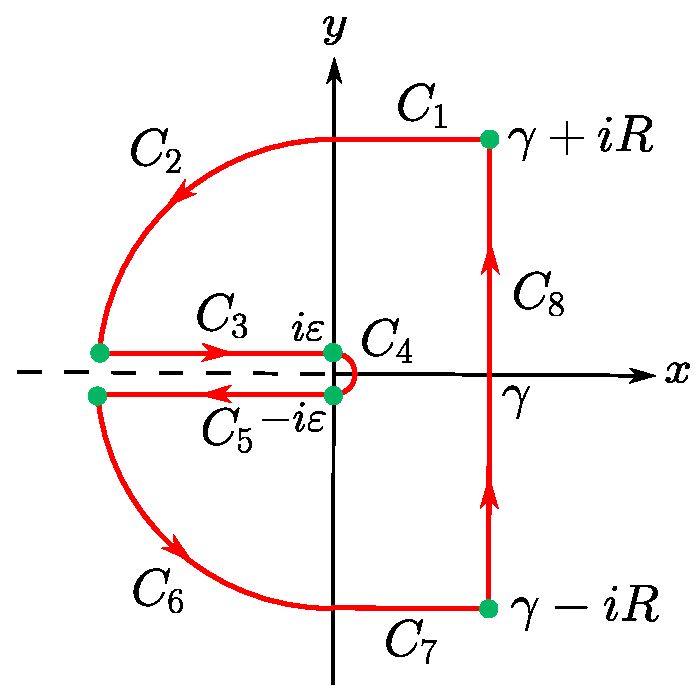
\includegraphics[scale = 0.6]{Figuras/InversaLaplace2.pdf}
        \caption{Contorno de integración para la transformada inversa de Laplace $1/\sqrt{s}$.}
        \label{fig:InvLaplaceBranchCut}
    \end{figure}

    Como el integrando es analítico en el interior del contorno cerrado, por el teorema de Cauchy-Goursat,
    $$\sum_{k=1}^{8} \int_{C_k} e^{st} \frac{1}{\sqrt{s}} \,ds = 0.$$

    Mostremos que la integral en torno a $C_1: s = x + i R, 0\leq x \leq \gamma$, se desvanece cuando $R \to \infty$. 

    Para $s \in C_1$, tenemos que
    $$\left|e^{st} \frac{1}{\sqrt{s}} \right| = \frac{e^{\real(s) t}}{\sqrt{|s|}} \leq \frac{e^{\gamma t}}{\sqrt{R}}.$$

    Luego,
    $$\left|\int_{C_1} e^{st} \frac{1}{\sqrt{s}} \,ds \right| \leq \int_0^{\gamma} \frac{e^{\gamma t}}{\sqrt{R}} \,dx = \frac{\gamma e^{\gamma t}}{\sqrt{R}} \overset{R \to \infty}{\longrightarrow} 0.$$

    Similarmente, se prueba que la integral en torno a $C_7: s = x - i R, 0 \leq x \leq \gamma$, se desvanece cuando $R \to \infty$.

    Ahora, mostremos que la integral en torno a $C_2: s = Re^{i\theta}, \pi/2 \leq \theta < \pi$, se desvanece cuando $R \to \infty$. 

     Para $s \in C_2$, tenemos que
    $$\left|e^{st} \frac{1}{\sqrt{s}} \right| = \frac{e^{\real(s) t}}{\sqrt{|s|}} = e^{R t \cos \theta }\frac{1}{\sqrt{R}}.$$

    Luego,
    $$\left|\int_{C_2} e^{st} \frac{1}{\sqrt{s}} \,ds \right| \leq \frac{1}{\sqrt{R}} \int_{\pi/2}^{\pi} e^{Rt \cos \theta} d\theta.$$

    Haciendo la sustitución $\phi = \theta - (\pi/2) \Rightarrow d\phi = d\theta$, en la integral y usando la desigualdad de Jordan, obtenemos
    $$\left|\int_{C_2} e^{st} \frac{1}{\sqrt{s}} \,ds \right| \leq \frac{1}{\sqrt{R}} \int_{0}^{\pi/2} e^{-Rt \sin \phi} d\phi \leq \frac{1}{\sqrt{R}} \frac{\pi}{2 R t}\overset{R \to \infty}{\longrightarrow} 0.$$

    Similarmente, se prueba que la integral en torno a $C_6$ se desvanece.

    Podemos mostrar que la integral en torno a $C_4: s = \varepsilon e^{i\theta}, -\pi/2 \leq \theta \leq \pi/2$, se desvanece cuando $\varepsilon \to 0$.

    Para $s \in C_4$, tenemos que
    $$\left|e^{st} \frac{1}{\sqrt{s}} \right| = \frac{e^{\real(s) t}}{\sqrt{|s|}} = \frac{e^{\varepsilon t \cos\theta}}{\sqrt{\varepsilon}} \leq  \frac{e^{\varepsilon t}}{\sqrt{\varepsilon}}.$$

    Luego,
    $$\left|\int_{C_4} e^{st} \frac{1}{\sqrt{s}} \,ds \right| \leq \frac{e^{\varepsilon t}}{\sqrt{\varepsilon}} \int_{-\pi/2}^{ \pi/2} \varepsilon d\theta = \frac{e^{\varepsilon t}}{\sqrt{\varepsilon}} (\pi \varepsilon) \overset{\varepsilon \to 0}{\longrightarrow} 0.$$

    Entonces,
    $$\int_{C_3} e^{st} \frac{1}{\sqrt{s}} \,ds + \int_{C_5} e^{st} \frac{1}{\sqrt{s}} \,ds + \int_{C_8} e^{st} \frac{1}{\sqrt{s}} \,ds = 0.$$

    Tomando el límite $R \to \infty$ y $\varepsilon \to 0$, podemos expresar la transformada inversa de Laplace como
    $$\mathcal{L}^{-1}\left\{ \frac{1}{\sqrt{s}}\right\} = \frac{1}{2\pi i} \int_{\gamma - i\infty}^{\gamma + i \infty} e^{st} \frac{1}{\sqrt{s}} \,ds = - \frac{1}{2\pi i} \lim_{R\to\infty}  \lim_{\varepsilon \to 0} \left[ \int_{C_3} e^{st} \frac{1}{\sqrt{s}} \,ds +  \int_{C_5} e^{st} \frac{1}{\sqrt{s}} \,ds\right].$$

    Bajo estos límites, tenemos que en $C_3$, $s = x$, $ds = dx$, con $x$ desde $-\infty$ a $0$, y en $C_5$, $s = x$, $ds = dx$, con $x$ desde $0$ a $-\infty$.  Luego,
    \begin{align*}
       \mathcal{L}^{-1}\left\{ \frac{1}{\sqrt{s}}\right\} &= - \frac{1}{2\pi i} \int_{-\infty}^0 e^{xt} \frac{e^{-i\pi/2}}{\sqrt{-x}} \,dx - \frac{1}{2\pi i} \int_0^{-\infty} e^{xt} \frac{e^{i\pi/2}}{\sqrt{-x}} \,dx \\
       &= -\frac{1}{2\pi} \int_{\infty}^0 e^{-xt} \frac{1}{\sqrt{x}} \,dx + \frac{1}{2\pi} \int_0^{\infty} e^{-xt} \frac{1}{\sqrt{x}} \,dx \\
       &= \frac{1}{\pi} \int_0^{\infty} e^{-xt} \frac{1}{\sqrt{x}} \,dx.
    \end{align*}

    Haciendo la sustitución $u = xt \Rightarrow du = t dx$,
    $$ \mathcal{L}^{-1}\left\{ \frac{1}{\sqrt{s}}\right\}  = \frac{1}{\pi \sqrt{t}} \int_0^{\infty} e^{-u} \frac{1}{\sqrt{u}} \,du.$$

    Pero,
    $$\int_0^{\infty} e^{-u} \frac{1}{\sqrt{u}} \,du = \Gamma\left( \frac{1}{2}\right) = \sqrt{\pi}.$$

    Por lo tanto,
    $$ \mathcal{L}^{-1}\left\{ \frac{1}{\sqrt{s}}\right\} = \frac{1}{\sqrt{\pi t}}, \quad t > 0.$$
\end{ejemplo}

\section{Propiedades de la transformada de Laplace}    

\begin{teorema}
    Si $f$ y $g$ son funciones cuyas transformadas de Laplace existen para $\real(s) > \alpha$ y sean $a, b \in \mathbb{R}$. Entonces, 
\begin{enumerate}
    \item \textbf{Linealidad:} Para $\real(s) > \alpha$,
    $$\mathcal{L}\{a f(t) + b g(t)\} = a \mathcal{L}\{f(t)\} + b \mathcal{L}\{g(t)\}.$$ 

    \item \textbf{Escalonamiento:} Para $\real(s) > \alpha \cdot \beta$,
    $$\mathcal{L}\{f(\beta t) \} = \frac{1}{\beta} F \left( \frac{s}{\beta}\right), \quad \beta > 0.$$ 
    
    \item \textbf{Desplazamiento en el plano $s$:} Para $\real(s) > \alpha + a$,
    $$\mathcal{L}\{e^{at} f(t)\} = F(s-a).$$
\end{enumerate}
\end{teorema}

\begin{ejemplo}
    Determine la transformada de Laplace de $e^{at} \sin(bt)$.

    \textbf{Solución:} En la primera sección, vimos que
    $$\mathcal{L}\{\sin(bt)\} = F(s) = \frac{b}{s^2+b^2}, \quad \real(s) > 0.$$

    Luego, por la propiedad de desplazamiento,
    $$\mathcal{L}\{e^{at} \sin(bt)\} = F(s-a) = \frac{b}{(s-a)^2+b^2}, \quad \real(s) > a.$$
\end{ejemplo}

\begin{teorema}[Propiedad de la derivada]
    Sea $f$ continua en $]0, + \infty [$ y $f'(t)$ continua por tramos en $[0, + \infty[$, ambas de orden exponencial $\alpha$. Entonces, para $\real(s) > \alpha$,
    $$\mathcal{L}\{f'(t)\} = s \mathcal{L}\{f(t)\} - f(0^+),$$

    donde $f(0^+) = \lim\limits_{t \to 0^+} f(t)$. 
\end{teorema}

En general, la transformada de Laplace de derivadas de orden superior están dadas por el siguiente teorema.

\begin{teorema}[Transformada de Laplace de derivadas de orden superior]
 Sean $f, f', \dots, f^{(n-1)}$ continuas para todo $t>0$ y sea $f^{(n)}$ continua por tramos en $[0,+\infty[$, con todas estas funciones de orden exponencial $\alpha$. Entonces, para $\real(s) > \alpha$,
$$\mathcal{L}\{f^{(n)}(t)\} = s^n \mathcal{L}\{f(t)\} - s^{n-1} f(0^+) - s^{n-2} f'(0^+) - \cdots - f^{(n-1)}(0^+). \label{LaplaceDerivada}$$

\end{teorema}

\begin{ejemplo}
Calcule 
$$\mathcal{L}\left\{\sin^2(at)\right\}.$$   

\textbf{Solución:} Sea $f(t) = \sin^2(at)$, entonces
$$f'(t) = 2a \sin(at) \cos(at) = a \sin(2at).$$

Como $f(0) = 0$ y $\frac{2a^2}{s^2+4a^2} = \mathcal{L}\{f'(t)\} = s \mathcal{L}\{f(t)\} - f(0)$, obtenemos
$$\mathcal{L}\left\{\sin^2(at)\right\} = \frac{2a^2}{s(s^2+4a^2)}, \quad \real(s) > 0.$$
\end{ejemplo}

Hemos determinando la transformada de Laplace de la derivada de una función $f$, es natural preguntarse sobre la transformada de una función definida por una integral:
$$g(t) = \int_0^t f(t') \,dt'.$$

\begin{teorema}
     Sea la función $f(t)$ continua por tramos y de orden exponencial $\alpha$. Entonces,
     $$\mathcal{L} \left\{ \int_0^t f(t') \,dt'\right\} = \frac{1}{s} \mathcal{L}\{f(t)\}, \quad \real(s) > \alpha.$$
\end{teorema}

\begin{demo}
Caso particular del teorema \ref{Teo:Convolucion} para 
$$(f * g)(t) = \int_0^t f(u) g(t-u) \,du,$$

con $g(t) = 1$.
\end{demo}

Para funciones periódicas, tenemos el siguiente teorema.

\begin{teorema}
 Sea $f$ una función continua por tramos en el intervalo $[0,T]$ y periódica con periodo $T>0$. Entonces $f$ tiene transformada de Laplace dada por
\begin{equation*}
\mathcal{L}\{f(t)\} = \frac{\int_0^T e^{-st} f(t) dt}{1-e^{-Ts}}, \quad \real(s) > 0.
\end{equation*}
   
\end{teorema}

\begin{ejemplo}
    Encuentre la transformada de Laplace de
    $$f(t) = \left\{ \begin{array}{cl}
     1,& \text{si} ~ 0 \leq t < \pi  \\
     0,& \text{si} ~ \pi \leq t < 2\pi
    \end{array} \right.$$

    y $f(t+ 2\pi) = f(t)$ para $t > 0$, ésto es, $f(t)$ es periódica para $t > 0$.

    \textbf{Solución:} Como $f$ es periódica de periodo $T = 2\pi$, tenemos que
    \begin{align*}
        \mathcal{L}\{f(t)\} &= \frac{\int_0^{2\pi} e^{-st} f(t) \,dt}{1-e^{-2\pi s}} \\
        &= \frac{\int_0^{\pi} e^{-st}\,dt}{1-e^{-2\pi s}} \\
        &= \frac{1-e^{-\pi s}}{s(1-e^{-2\pi s})} \\
        &= \frac{1}{s(1+e^{-\pi s})}.
    \end{align*}
\end{ejemplo}

\begin{teorema}[Integral de una transformada]
   Si $\int_0^{\beta} \frac{f(t)}{t} \,dt$ existe para $\beta > 0$ y $f(t)$ es de orden exponencial $\alpha$, entonces
   $$\mathcal{L}\left\{\frac{f(t)}{t}\right\} = \int_s^{\infty} F(u) \,du, \quad s > \alpha.$$
\end{teorema}

\section{Convolución}

\begin{defi}
   Sean $f$ y $g$ funciones continuas por tramos en $[0, \infty[$. La \textbf{convolución} de $f$ y $g$, que se denota $f*g$, se define como
\begin{equation*}
(f*g)(t) := \int_0^t f(t-u)g(u) \, du.
\end{equation*}  
\end{defi}

Es claro que la convolución es distinta de la multiplicación común. Por ejemplo, $1*1 = t \neq 1$, y en general, $1*f \neq f$. Sin embargo, la convolución sí satisface algunas propiedades de la multiplicación.

\begin{teorema}[Propiedades de la convolución]
Sean $f$, $g$ y $h$ continuas por tramos en $[0,  \infty[$. Entonces,

\begin{itemize}
\item[(i)] $f*g = g*f$,

\item[(ii)] $f*(g*h) = (f*g)*h$,  

\item[(iii)] $f*(g+h) = f*g + f*h$. 
\end{itemize} 
\end{teorema}

Al igual que para la transformada de Fourier, la transformada de Laplace de la convolución obedece el siguiente teorema.

\begin{teorema}[de Convolución] \label{Teo:Convolucion}
    Sean $f$ y $g$ funciones continuas por tramos, de orden exponencial, tales que:
    \begin{equation*}
    \mathcal{L}\{f(t)\} = F(s) ~~\mbox{y}~~ \mathcal{L}\{g(t)\} = G(s),
    \end{equation*}

    entonces
    \begin{equation*}
    \mathcal{L}\{(f*g)(t)\} = F(s)G(s),
    \end{equation*}

    o, de manera equivalente,
    \begin{equation*}
    \mathcal{L}^{-1}\{F(s)G(s)\}(t) = (f*g)(t).
    \end{equation*}    
\end{teorema}

\begin{demo}

Tomando la transformada de Laplace de la convolución $f * g$,
$$\mathcal{L}\{(f*g)(t)\} = \int_0^{\infty} e^{-st} \int_0^t f(t-u) g(u) \,du \,dt = \int_0^{\infty} \int_0^t e^{-st}  f(t-u) g(u) \,du \,dt.$$

La región de integración se ilustra en la figura \ref{fig:Convolucion2}.

\begin{figure}[H]
    \centering
    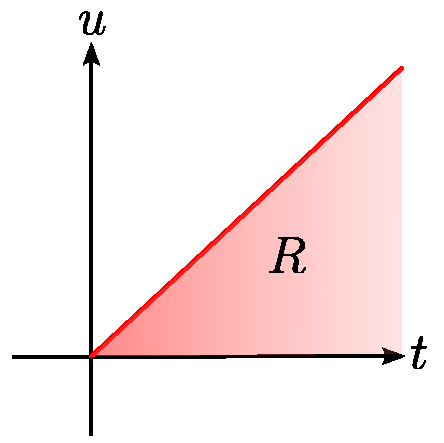
\includegraphics[scale = 0.6]{Figuras/Laplace-Convolucion-2.pdf}
    \caption{Región de integración.}
    \label{fig:Convolucion2}
\end{figure}

Luego, haciendo un cambio en el orden de integración, se tiene
$$\mathcal{L}\{(f*g)(t)\} = \int_0^{\infty} \int_u^{\infty} e^{-st} f(t-u) g(u) \,dt\,du.$$

Si hacemos el cambio de variable $v = t-u$ en la integral interior, obtenemos que
\begin{align*}
    \mathcal{L}\{(f*g)(t)\} &= \int_0^{\infty} g(u) \int_0^{\infty} e^{-s(u+v)} f(v) \,dv \,du \\
    &= \left(\int_0^{\infty} g(u) e^{-su} du \right)\left(\int_0^{\infty} f(v) e^{-sv} \,dv  \right) \\
    &= F(s)G(s). 
\end{align*}

\end{demo}

\begin{ejemplo}
Calcule
$$\mathcal{L}^{-1} \left\{ \frac{s}{(s^2+1)^2} \right\}.$$

\textbf{Solución:} Notemos que 
\begin{equation*}
\mathcal{L}^{-1} \left\{ \frac{s}{(s^2+1)^2} \right\} = \mathcal{L}^{-1} \left\{ \frac{s}{s^2+1} \cdot \frac{1}{s^2+1} \right\}.
\end{equation*}

Como
\begin{equation*}
\mathcal{L}\{\cos(t)\} = \frac{s}{s^2+1} ~~\mbox{y}~~ \mathcal{L}\{\sin(t)\} = \frac{1}{s^2+1},
\end{equation*}

tenemos, por el teorema de convolución, que
\begin{align*}
    \mathcal{L}^{-1} \left\{ \frac{s}{(s^2+1)^2} \right\} &=\cos(t) *\sin(t)  \\
    &= \int_0^t \sin(t-u) \cos(u) \,du \\
    &= \int_0^t (\sin(t) \cos(u) - \cos(u) \sin(u)) \cos(u) \,du  \\
    &= \sin(t) \int_0^t \cos^2(u) \,du - \cos(t) \int_0^t \sin (u) \cos(u) \,du \\
    &= \sin(t) \left[ \frac{1}{2} u + \frac{\sin(2u)}{4} \right]_0^t - \cos(t) \left[ \frac{\sin^2(u)}{2} \right]_0^t \\
    &= \frac{t \sin(t)}{2} + \frac{\sin(2t)}{4} \sin(t) - \cos(t) \frac{\sin^2(t)}{2} \\
    &= \frac{t \sin(t) }{2}.
\end{align*}

Por lo tanto,
$$\mathcal{L}^{-1} \left\{ \frac{s}{(s^2+1)^2} \right\} = \frac{t \sin(t) }{2}.$$   
\end{ejemplo}

\section{Aplicaciones de la transformada de Laplace}

La transformada de Laplace, al igual que la transformada de Fourier, nos permite convertir ecuaciones diferenciales en ecuaciones algebraicas, con una diferencia: se requiere el valor de la función en un punto dado. Lo anterior nos entrega una ligera ventaja y es que una vez que se invierta la transformada, tendremos de inmediato la solución al problema, recalcando que el dominio de validez de la función encontrada es para $t > 0$. Otra diferencia relevante es que, mientras la transformada de Fourier sólo se puede aplicar a funciones que decrecen rápidamente a cero, la transformada de Laplace está bien definida incluso para funciones de crecimiento exponencial. Entonces, si estamos en presencia de un sistema físico caracterizado por una variable que crece exponencialmente, es bastante probable que la transformada de Fourier dé resultados sin sentido físico.

A continuación expondremos tres situaciones, en las cuales el uso de la transformada de Laplace es ventajoso.

\subsection{Ecuaciones diferenciales lineales con coeficientes constantes}

\begin{ejemplo}
    Consideremos la ecuación diferencial
    $$y'(t) + y(t) = \cos(t), \quad \text{para} ~ t > 0, \quad y(0) = 1.$$

    Apliquemos la transformada de Laplace a ambos lados de la ecuación:
    $$\mathcal{L}\{y'(t)\} - \mathcal{L}\{y(t)\} = \mathcal{L}\{\cos(t)\}.$$

    Evaluamos la transformada de la primera derivada, usando los teoremas enunciados durante el capítulo.
    $$\mathcal{L}\{y'(t)\} = s Y(s) - y(0) = s Y(s) - 1,$$

    donde $Y(s) = \mathcal{L}\{y(t)\}$. Luego, la ecuación diferencial nos queda:
    \begin{align*}
        sY(s) - 1 + Y(s) &= \frac{s}{s^2+1} \\
        \Rightarrow \quad Y(s) &= \frac{s}{(s+1)(s^2+1)} + \frac{1}{s+1} \\
        \Rightarrow \quad Y(s) &= \frac{1/2}{s+1} + \frac{1}{2} \frac{s+1}{s^2+1}.
    \end{align*}

    Aplicando la transformada de Laplace inversa,
    $$y(t) = \frac{1}{2} e^{-t} + \frac{1}{2} \cos(t) + \frac{1}{2} \sin(t), \quad t > 0.$$
\end{ejemplo}

\subsection{Ecuaciones integrales}

Una \textbf{ecuación integral} es aquella ecuación donde la función incógnita $\varphi(x)$ se encuentra dentro de una integral. Estas ecuaciones integrales se clasifican en dos formas \cite{Arfken}:
\begin{itemize}
    \item Si los límites de integración están fijos, llamamos la ecuación una \textbf{ecuación de Fredholm}; si un límite es variable, es una \textbf{ecuación de Volterra}.

    \item Si la función incógnita aparece solo en la integral, la etiquetamos como de \textbf{primera especie}. Si aparece tanto dentro como fuera de la integral, la etiquetemos como de \textbf{segunda especie}.
\end{itemize}

A continuación algunos ejemplos de estas definiciones donde $\varphi(t)$ es la función desconocida, $K(x,t)$ una función de dos variables que la llamaremos \textbf{kernel}, y $f(x)$ una función que asumimos conocida.

\begin{enumerate}
    \item \textbf{Ecuación de Fredholm de primera especie}:
    $$f(x) = \int_a^b K(x,t) \varphi(t) \,dt.$$

    \item \textbf{Ecuación de Fredholm de segunda especie}:
    $$\varphi(x) = f(x) + \lambda \int_a^b K(x,t) \varphi(t) \,dt.$$

    \item \textbf{Ecuación de Volterra de primera especie}:
    $$f(x) = \int_a^x K(x,t) \varphi(t) \,dt.$$

    \item \textbf{Ecuación de Volterra de segunda especie}:
    $$\varphi(x) = f(x) + \int_a^x K(x,t) \varphi(t) \,dt.$$
\end{enumerate}

En esta sección nos enfocaremos en ecuaciones de Volterra para $K(x,t) = K(x-t)$, de tal forma que
$$\int_a^x K(x,t) \varphi(t) \,dt = (K * \varphi)(x).$$

Para ilustrar el método, consideremos la situación física planteada en el siguiente ejemplo.

\begin{ejemplo}[Problema de la tautócrona]
    Una partícula de masa $m$ resbala (parte del reposo), sin roce, sobre una curva bajo el efecto de la gravedad. Buscamos determinar la forma de la curva de modo que el tiempo que le toma a la partícula en llegar al suelo sea independiente del punto de lanzamiento. 

    \begin{figure}[H]
        \centering
        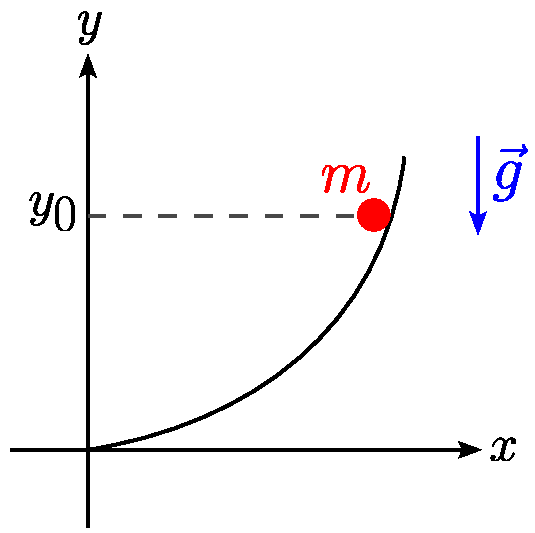
\includegraphics[scale = 0.65]{Figuras/tautocrona.pdf}
        \caption{Esquema de la situación física.}
        \label{fig:tautocrona}
    \end{figure}

    Como estamos en presencia de fuerzas conservativas, la  energía se conserva durante todo el trayecto para todo $y$, ésto es,
    \begin{alignat*}{3}
    &               &\quad   \text{Energía inicial en $y_0$} &= \text{Energía final en $y$} \\
    &  \Rightarrow  &\quad      mgy_0 &= \frac{1}{2} mv^2 + mgy \\
    &  \Rightarrow  &\quad   \frac{1}{2} mv^2 &= mg(y_0 - y) \\
    &  \Rightarrow  &\quad   v &= \sqrt{2 g} \sqrt{y_0-y}, 
    \end{alignat*}   
    
    donde $y_0$ es la altura inicial. El tiempo de descenso está dado por
    $$T(y_0) = \int \frac{ds}{v} = \int_{y_0}^0 \frac{1}{v} \frac{ds}{dy} dy = - \int_0^{y_0} f(y) (y_0 - y)^{-1/2} \frac{1}{\sqrt{2g}} dy,$$

    donde $f(y) = ds/dy$. Ahora, si suponemos que $T(y_0)$ es constante $T_0$, ésto es, independiente del punto de partida $y_0$. La condición queda
    $$\int_0^{y_0} f(y) (y_0 - y)^{-1/2} \,dy = C_0,$$

    donde $C_0 = -\sqrt{2g} T_0$. Aplicando la transformada de Laplace  a ambos lados de la ecuación:
    $$\mathcal{L}\left\{\int_0^{y_0} f(y) (y_0 - y)^{-1/2} \,dy \right\} = \mathcal{L}\{C_0\} = \frac{C_0}{s}.$$
    
    Por el teorema de convolución, tenemos que
    $$\mathcal{L}\{f(y)\} \mathcal{L}\{y^{-1/2}\} = \frac{C_0}{s} \Rightarrow \mathcal{L}\{f(y)\} = \frac{C_0/s}{\mathcal{L}\{y^{-1/2}\}}.$$

    Pero,
    $$\mathcal{L}\{y^{-1/2}\} = \int_0^{\infty} e^{-sy} \frac{1}{\sqrt{y}} \,dy \overset{\textcolor{blue}{t = sy}}{=} \frac{1}{\sqrt{s}}\int_0^{\infty} e^{-t} \frac{1}{\sqrt{t}} \,dt = \frac{\Gamma\left(\frac{1}{2}\right)}{\sqrt{s}}.$$

    Así,
    $$\mathcal{L}\{f(y)\} = \frac{C_0}{s} \frac{\sqrt{s}}{\Gamma\left(\frac{1}{2}\right)} = \frac{C_0}{\sqrt{\pi}} \frac{1}{\sqrt{s}}.$$

    Tomando la transformada inversando y usando el resultado del ejemplo \ref{Inv_Laplace_ej_branch}, obtenemos 
    $$f(y) = \frac{C_0}{\pi} \frac{1}{\sqrt{y}} = \frac{C}{\sqrt{y}},$$

    donde $C = C_0/\pi$. Recordando que $f(y) = ds/dy$, notemos que
    \begin{align*}
        ds^2 = dx^2 + dy^2 &\Rightarrow dx = \sqrt{ds^2 - dy^2} \\
        &\Rightarrow dx = \sqrt{\left( \frac{ds}{dy} dy\right)^2 - dy^2} \\
        &\Rightarrow dx = \sqrt{\left(\frac{ds}{dy}\right)^2 - 1} \,dy \\
        &\Rightarrow \frac{dx}{dy} = \sqrt{\frac{C^2}{y} - 1}. 
    \end{align*}

    Integrando con respecto a $y$,
    $$x(y) = \int \sqrt{\frac{C^2}{y} - 1} \,dy.$$

    Haciendo el cambio de variable $y = C^2 \sin^2 (\phi) \Rightarrow dy = 2 C^2 \sin(\phi) \cos(\phi) \,d\phi$,
    \begin{align*}
        x &= \int \sqrt{\csc^2(\phi) - 1} \, 2 C^2 \sin(\phi) \cos(\phi) \,d\phi \\
        &= 2C^2 \int \sqrt{\cot^2(\phi)}  \sin(\phi) \cos(\phi) \,d\phi \\
        &= 2C^2 \int \cos^2(\phi) \,d\phi \\
        &=  \frac{C^2}{2} (2\phi + \sin(2\phi)) + D,
    \end{align*}

    donde $D$ es una constante de integración. Entonces,
    \begin{align*}
        x &= \frac{C^2}{2} (2\phi + \sin(2\phi)) + D, \\
        y &= \frac{C^2}{2} (1 - \cos(2\phi)).
    \end{align*}

    La curva debe pasar por el origen $(0,0)$, así que $D = 0$, y si definimos un nuevo parámetro $\theta = 2\phi$, encontramos que
    \begin{align*}
        x &= \frac{C^2}{2} (\theta + \sin(\theta)), \\
        y &= \frac{C^2}{2} (1 - \cos(\theta)).
    \end{align*}

    Estas son las ecuaciones paramétricas de un cicloide.
\end{ejemplo}

\subsection{Sistema de ecuaciones lineales}

La transformada de Laplace puede ser usada para convertir un sistema de ecuaciones diferenciales con coeficientes constantes en un sistema de ecuaciones algebraicas. 

\begin{ejemplo}
    Consideremos el circuito de la figura \ref{fig:Circuit}. 
    
    \begin{figure}[H]
        \centering
        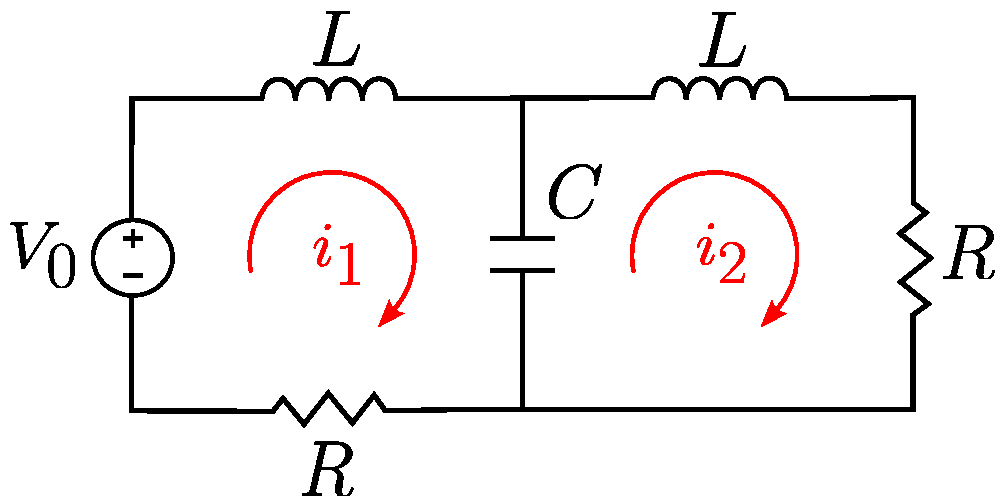
\includegraphics[scale = 0.65]{Figuras/Circuito.pdf}
        \caption{Circuito eléctrico.}
        \label{fig:Circuit}
    \end{figure}
    
    Usando las leyes de Kirchhoff, encontramos el siguiente sistema de ecuaciones diferenciales.
    \begin{align*}
        L \frac{di_1}{dt} + Ri_1 + \frac{q}{C} &= V_0, \\
        L \frac{di_2}{dt} + Ri_2 - \frac{q}{C} &= 0, \\
        \frac{dq}{dt} &= i_1 - i_2.
    \end{align*}
    
    Inicialmente el capacitador se encuentra descargado y las corrientes inducidas por las inductancias son despreciables de tal forma que se tienen las condiciones iniciales:
    $$i_1(0) = i_2(0) = \frac{V_0}{2R}, \quad q(0) = 0.$$

    Aplicamos la transformada de Laplace al sistema de ecuaciones diferenciales.
    \begin{align*}
        L\left( sI_1(s) - \frac{V_0}{2R} \right) + RI_1(s) + \frac{Q(s)}{C} &= \frac{V_0}{s}, \\
       L\left( sI_2(s) - \frac{V_0}{2R} \right) + RI_2(s) - \frac{Q(s)}{C}  &= 0, \\
        sQ(s) &= I_1(s) - I_2(s),
    \end{align*}

    donde $I_1(s) = \mathcal{L}\{i_1(t)\}$, $I_2(s) = \mathcal{L}\{i_2(t)\}$ y $Q(s) = \mathcal{L}\{q(t)\}$. Despejando estas cantidades:
    \begin{align*}
        I_1 &= \frac{V_0}{2} \left(\frac{1}{Rs} + \frac{1/L}{s^2 + R s/L + 2/(CL)} \right) \\
        I_2 &= \frac{V_0}{2} \left(\frac{1}{Rs} - \frac{1/L}{s^2 + R s/L + 2/(CL)} \right) \\
            Q &= \frac{C V_0}{2} \left( \frac{1}{s} - \frac{s+R/L}{s^2 + Rs/L + 2/(CL)} \right)
    \end{align*}

    Factorizando las polinomios de los denominadores.
    \begin{align*}
        I_1 &= \frac{V_0}{2} \left(\frac{1}{Rs} + \frac{1/L}{(s+\alpha - i \omega)(s + \alpha + i \omega)} \right) \\
        I_2 &= \frac{V_0}{2} \left(\frac{1}{Rs} - \frac{1/L}{(s+\alpha - i\omega)(s+\alpha + i \omega)} \right) \\
        Q &= \frac{C V_0}{2} \left( \frac{1}{s} - \frac{s+2\alpha}{(s+\alpha - i\omega)(s+\alpha + i \omega))} \right).
    \end{align*}

    Aquí hemos definido
    $$\alpha = \frac{R}{2L} \quad \text{y} \quad \omega^2 = \frac{2}{LC} - \alpha^2.$$

    Expandiendo las funciones en fracciones parciales.
    \begin{align*}
        I_1 &= \frac{V_0}{2} \left(\frac{1}{Rs} + \frac{i}{2\omega L} \left(\frac{1}{s+\alpha + i\omega} - \frac{1}{s+\alpha - i\omega} \right) \right) \\
        I_2 &= \frac{V_0}{2} \left(\frac{1}{Rs} - \frac{i}{2\omega L} \left(\frac{1}{s+\alpha + i\omega} - \frac{1}{s+\alpha - i\omega} \right) \right) \\
        Q &= \frac{C V_0}{2} \left( \frac{1}{s} + \frac{i}{2\omega} \left( \frac{\alpha + i\omega}{s+\alpha - i\omega} - \frac{\alpha - i \omega}{s+\alpha +i\Omega} \right) \right).
    \end{align*}

    Ahora, aplicamos la transformada inversa, teniendo en consideración que
    $$\mathcal{L}^{-1}\left\{ \frac{1}{s-a} \right\} = e^{at},$$
     \begin{align*}
        i_1 &= \frac{V_0}{2} \left(\frac{1}{R} + \frac{i}{2\omega L} \left( e^{(-\alpha - i\omega)t} - e^{(-\alpha + i\omega)t}\right) \right) \\
        i_2 &= \frac{V_0}{2} \left(\frac{1}{R} - \frac{i}{2\omega L} \left( e^{(-\alpha - i\omega)t} - e^{(-\alpha + i \omega)t}\right) \right) \\
        q &= \frac{C V_0}{2} \left( 1 + \frac{i}{2\omega} \left( (\alpha + i\omega) e^{(-\alpha + i \omega)t} - (\alpha - i\omega)e^{(-\alpha - i\omega)t} \right) \right).
    \end{align*}

    Simplicando las expresiones, obtenemos las soluciones.
    \begin{align*}
        i_1 &= \frac{V_0}{2} \left(\frac{1}{R} + \frac{1}{\omega L} e^{-\alpha t}\sin(\omega t) \right), \\
        i_2 &= \frac{V_0}{2} \left(\frac{1}{R} - \frac{1}{\omega L} e^{-\alpha t}\sin(\omega t) \right), \\
        q &= \frac{CV_0}{2} \left( 1- e^{-\alpha t} \left( \cos(\omega t) + \frac{\alpha}{\omega} \sin(\omega t) \right)\right).
    \end{align*}
\end{ejemplo}








 
